% Chapter 8

\chapter{Implementation of the analysis using XMG} % Write in your own chapter title
\label{Chapter8}
%\lhead{Chapter 7. \emph{Implementation of analysis using XMG}} 
In Chapter~\ref{Chapter7} I have proposed a frame \isi{semantic analysis} of various prefixes together with selected pieces of the \isi{syntax-semantics interface}. In this chapter I present the implementation of the proposal.

 In order to describe and provide a compact grammar description, one can use a \isi{metagrammar} compiler. A TAG \isi{metagrammar} is a reduced description that captures linguistic generalisations that appear in the trees that belong to the grammar \citep{Candito:99}. EXtensible MetaGrammar\footnote{\url{http://xmg.phil.hhu.de/}} \citep[\isi{XMG},][]{Crabbe:13} is a formalism that allows to describe linguistic information contained in the grammar and a tool to compute grammar rules and produce a redundant strongly lexicalised TAG. 
 
Among the properties of \isi{XMG} that distinguish it from other grammar engineering environments, two are of particular importance for the current work. First, \isi{XMG} is a declarative language, which means that it is based on constraints and not on procedures. This allows for an order-independent definition of grammaticality. Second, \isi{XMG}'s notation is highly expressive: in particular, various linguistic dimensions are treated in a modular war, and grammatical units can be disjoint, conjoint, and inherited.
 
 \isi{XMG} 2 \citep{Petitjean:16} is a tool that is used to create \isi{metagrammar} compilers, adapting them to specific needs. Whereas \isi{XMG} supports three independent levels of description: \isi{syntactic trees} (syn), semantic predicate structures (sem), and dynamic interfaces between syn and sem (dyn), \isi{XMG} 2 allows to introduce additional dimensions. The compiler I am using for the current implementation is created using \isi{XMG} 2 and has a syntactic (syn) and a frame semantic (frame) dimension  \citep{Lichte:15}.

The syntactic dimension is described using the following elements: first, all the nodes are declared using the keyword \texttt{node} and a variable name. These declarations are accompanied by optional marks (in brackets) and syntactic features (in square brackets, separated by commas). Values of syntactic features can be either specified or represented by a variable to ensure the same value of the feature across the nodes without specifying it. Second, the relations between the nodes are stated. I will use the following relations ($x$ and $y$ range over node variables): $x \rightarrow y$ for the immediate dominance of the node $x$ over the node $y$; $x \rightarrow + y$ for the dominance (reflexive transitive closure of the immediate dominance relation) of the node $x$ over the node $y$; 
$x >> y$ for the immediate precedence of the node $x$; and $x >>+ y$ for the precedence (transitive closure of the immediate precedence relation) of the node $x$.

\isi{XMG} is designed to output unanchored TAG elementary trees, but as currently there is no parser that would take into account frame semantic dimension, I simulate the insertion of \isi{lexical anchors} in the \isi{metagrammar}. This solution leads to a more complicated \isi{metagrammar} architecture, but allows to see the results in a form that can be easily understood. If I were to output the unanchored trees only, I would obtain \isi{prefixation} schemes but the stem that carries important information would not be inserted, which would make is very hard to check the predictions. 

%On the other hand, I had to limit the size of the fragment for implementation, as together with all the lexical decisions the \isi{metagrammar} descriptions grows too fast and it becomes harder to maintain and test it. 

The implemented grammar fragment I want to show contains the following elements: a noun \textit{rasskaz} `story', a verb \textit{pisat'} `to write', a prefixed verb \textit{zapisat'} `to write down', prefixes \Prefix{po-} (\isi{delimitative} and \isi{distributive} interpretations), \Prefix{pere-} (\isi{repetitive} and \isi{distributive} interpretations), and \Prefix{do-}, and \isi{imperfective suffix} \textit{-iva-} (iterative and progressive interpretations).  With this inventory I construct verbs with a maximum of four affixes (can be realised if the a base verb is prefixed two times, then suffixed, and then prefixed again). This architecture in principle allows to construct more than 1000 verbal phrases, out of which the compiler outputs 88 models. Nine of those models have to be filtered out later by the pragmatic module, but those numbers show that most of the work is done by the constraints from the syntax-semantics part.

In this chapter I will show fragments of the implementation and explain decisions that I had to make. The whole code and the corresponding output of the compiler are provided in Section~\ref{B:me} of Appendix~\ref{AppendixB}. In the last section I will present an implementation of the analysis proposed in \citet{Tatevosov:09} (code provided in Section~\ref{B:Tat} of Appendix~\ref{AppendixB}) that is done using the same tools. I will then compare the outputs of two implementations. Both implementations and the xml files that are output by the compiler are also available online\footnote{\url{https://user.phil-fak.uni-duesseldorf.de/~zinova/XMG/index.html}}.

\section{Type hierarchy and constraints}
The code starts with the three unicity constraints shown on \figref{xmg:unicity} that prevent the appearance of some features more than once in the same \isi{elementary tree}. The first constraint is a standard one, as it ensures that each tree has one \isi{lexical anchor}. The second constraint has to be introduced because I use \isi{XMG} not only for constructing the unanchored trees, but also for the insertion of the \isi{lexical anchors}. This constraint allows to make sure that only one noun is inserted in the accusative noun slot.

\begin{figure}
\begin{lstlisting}[style=xmg]
use unicity with (mark=anchor) dims (syn)
use unicity with (mark=nounacc) dims (syn)
use unicity with (iteration=yes) dims (syn)
\end{lstlisting}
\caption{XMG code: unicity constraints \label{xmg:unicity}}
\end{figure}

The third constraint restricts the appearance of the \textit{iteration} feature to one per tree. The nature of this constraint is semantic and the natural way would be to locate it in the semantic dimension. This is, however, not yet implemented, so I copy the feature to the syntactic level and apply the unicity constraint in the syntactic dimension.

The next three sections introduce syntactic features, types associated with values of these features, and frame types. Here I want to note two more features that I had to ``lift'' to the syntactic level due to the fact that such feature checking inside the semantic dimension of \isi{XMG} is not yet supported: \textit{bounded} and \textit{limited}. The feature \textit{bounded} appears at those nodes that are associated with frames of \textit{event} type. It gets the value \textit{yes} if there is a path from the central node of the frame to an attribute \FIN that can proceed through the \PARTOF attributes. If there is no such path, the value of the feature is \textit{no}. The feature \textit{limited} is a stronger version of a similar constraint: for \textit{limited} to get the value \textit{yes}, the central node has to have an attribute \FIN and its value has to be specific (concrete value or a bound variable). In all other cases the feature \textit{limited} gets value the \textit{no}.

We have discussed the crucial fragments of the \isi{type hierarchy} in Section~\ref{section:types}. Now all those restrictions plus some more constraints that are related to the nominal domain were left out from the previous discussion have to be formalised. Figure~\ref{xmg:types} shows a part of type constraints that states that \textit{length} is a type of \textit{scale}, in particular \textit{property-scale}. This type is not compatible with a \textit{cardinality} scale type which is always a \textit{closed-scale}. The rest of the hierarchy is written in a similar way.

\begin{figure}
\begin{lstlisting}[style=xmg]
property-scale -> scale,
length -> property-scale,
cardinality property-scale -> -,
closed-scale -> scale
cardinality -> closed-scale,
\end{lstlisting}
\caption{A fragment of type hierarchy \label{xmg:types}}
\end{figure}

\section{Lexical anchors}\largerpage[-1]
In a proper implementation that would separate the \isi{metagrammar} level from the syntactic level the following elements would not belong to the \isi{metagrammar}, but would be used as \isi{lexical anchors} for the appropriate tree families. The first entry is the noun that will be used to fill the object slot. I have selected the plural form of the noun \textit{rasskaz} `story' that has some length and also cardinality. The constraint on the unicity of the feature \textit{nounacc} that I have shown above is used here to prevent multiple insertions of the accusative noun \isi{lexical anchor}.

The description of the noun is straightforward: on the syntactic side, it is a daughter of the N category node and on the semantic side it contains relevant attributes. The two nodes (\texttt{?N} and \texttt{?Story}) are declared in the first two lines of the syntactic domain description and connected via an immediate dominance relation in the third line. Both nodes are characterised with feature \texttt{i=?X0} which connects them to the semantic frame characterised in the frame dimension. The frame description states that the type of the frame \texttt{?X0} is \texttt{story} and it has two attributes: The label of the central node of the frame (\texttt{?X0}) as well as the syntactic nodes and relevant dimension-related variables are exported for future use. 

The code for the class is shown on \figref{xmg:noun}. Note that I do not distinguish between top and bottom feature structures in the provided descriptions, as due to the absence of the \isi{adjunction} in the implemented fragment the division into top and bottom parts is not relevant. Figure~\ref{story:tree:frame} shows the tree and the frame that are described by the code for the class \texttt{Story} (features of the syntactic dimension are omitted).

\begin{figure}[p]
\begin{lstlisting}[style=xmg,basicstyle=\small\ttfamily]
class Story
export ?Length ?Card ?N
declare ?N ?Story ?X0 ?Length ?Card
{
  <syn>{
    node ?N (mark=coanchor) [cat=n, num = pl, i=?X0];
    node ?Story (mark=nounacc) [cat=rasskazy, num = pl, i=?X0];
    ?N -> ?Story
  };
  <frame>{
    ?X0[story,
        length: ?Length,
        cardinality: ?Card
    ]
  }
}
\end{lstlisting}
\caption{XMG code: noun that is used to fill the accusative NP slot \label{xmg:noun}}
\end{figure}

\begin{figure}[p]
\begin{minipage}{.5\textwidth}
\centering
% % 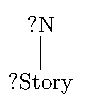
\includegraphics[scale=1]{StoryTree.pdf}
\begin{forest}
[?N [?Story]]
\end{forest}
\end{minipage}%
\begin{minipage}{0.5\textwidth}
\avm[types=\normalfont,values=\normalfont,attributes=\normalfont]{
?X0 [\type*{story}
      length & ?Length\\
      cardinality & ?Card
   ]}
\end{minipage}
\caption{Tree and frame representation of the code provided on \figref{xmg:noun}\label{story:tree:frame}}
\end{figure}\clearpage

Later this noun can enter one of the two \isi{dimension constructors}: length or cardinality. The \isi{cardinality constructor} code is shown on \figref{xmg:cardinality}. It should be available for all nouns that have a cardinality attribute with an additional restriction for plural number. The constructor creates a NP node that dominates the N node exported from the description of the noun, and a VP node that linearly precedes the NP node. The output of the class is a discontinuous tree, as shown by the tree on \figref{card:tree:frame}. On the semantic side an \MDIM attribute is created and the event description bounded to the VP node also acquires the type \textit{iteration}. This is, as announced before, doubled via the iteration attribute on the syntactic side. The frame described by the frame part of the code is provided on the right side of \figref{card:tree:frame}.

\vfil
\begin{figure}
\begin{lstlisting}[style=xmg,basicstyle=\small\ttfamily]
class NounCardinal
export ?N ?NP ?VP
declare ?NCard ?X0 ?Card ?N ?NP ?VP ?Dim ?Theme ?Case ?Num 
{
  ?NCard=Story[];
  ?NCard.?Card = ?Card;
  ?N=?NCard.?N;
    <syn>{
    node ?NP [cat=np, case=?Case, num = pl, i=?Theme];
    node ?VP [cat=vp, e=?X0, iteration = yes];
    node ?N (mark=coanchor) [cat=n, case = ?Case, num = pl, i=?Theme];
    ?VP >>+ ?NP;
    ?NP -> ?N
  };
  <frame>{
    ?X0[iteration,
        theme:?Theme,
        m-dim:[cardinality,
                min:[zero],
                max:?Card
        ]
    ]
  }
}
\end{lstlisting}
\caption{XMG code: constructor of the cardinality dimension \label{xmg:cardinality}}
\end{figure}
\vfil
\pagebreak

\begin{figure}
% \begin{minipage}{0.5\textwidth}
% % 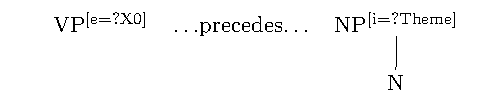
\includegraphics[scale=1]{NounCardTree.pdf}\\
\begin{tikzpicture}[baseline]
\node at (0,0) (VP) {\strut VP\textsuperscript{[e=?X0]}};
\node [right=.5cm of VP] (precedes) {...precedes...};
\node [right=.5cm of precedes] (NP) {\strut NP\textsuperscript{[i=?Theme]}};
\node [below=\baselineskip of NP] (N) {N};
\draw (NP) -- (N);
\end{tikzpicture}\medskip\\
% \end{minipage}%
% \begin{minipage}{0.5\textwidth}
\avm[types=\normalfont,values=\normalfont,attributes=\normalfont]{
?X0 [\type*{iteration}
      theme & ?Theme\\
      m-dim & [\type*{cardinality}
      	min & [\type{zero}]\\
      	max & ?Card]
]
}
% \end{minipage}
\caption{Tree and frame representation of the code provided on \figref{xmg:cardinality}\label{card:tree:frame}}
\end{figure}

Another dimension constructor that I use, implemented in the class \texttt{NounLength},  is organised in a similar way with a difference that it creates a \NOUNDIM, not an \MDIM attribute of the event, is available for nouns that have a \LENGTH attribute independently of their number, and does not specify the event type.

\begin{figure}
\begin{lstlisting}[style=xmg,basicstyle=\small\ttfamily]
class Pisat
export ?V
declare ?V ?Pisat ?X0 ?Actor ?Theme ?Mean
{
  <syn>{
    node ?V (mark=anchor) [cat=v, e=?X0, asp = unbound, aspect = imperf];
    node ?Pisat (mark=flex) [cat=pisat, e=?X0, asp = unbound, 
    	aspect = imperf];
    ?V -> ?Pisat
  }
  ;
  <frame>{
    ?X0[event & process,
        actor:?Actor,
        theme:?Theme,
        mean:?Mean,
        manner:[write],
        verb-dim:?X0
    ]
  }
}
\end{lstlisting}
\caption{XMG code for representation of the verb \textit{pisat'} `to write' \label{xmg:pisat}}
\end{figure}

The second group of lexical items consists of two verbs: \textit{pisat'} `to write' and \textit{zapisat'} `to write down'. The second verb contains the prefix \Prefix{za-}, but its semantic contribution is not transparent, so the whole verb must be stored in the dictionary. The class that represents the verb \textit{pisat'} `to write' has a simple \isi{syntactic structure} of two nodes (see \figref{xmg:pisat}): the node of category V and the node that contains the verb itself, where the V node inherits all syntactic properties of the verb, except for the category. The \textit{aspect} feature, in contrast with the features \textit{limited} and \textit{bounded}, is a syntactic feature and carries information about the syntactic aspect of the verb represented by the respective node. For the frame semantic side, I use a simple representation that serves the purposes of the current analysis. I acknowledge that the fully elaborated representation may be more complex or just differ in details, but this should not influence the results of the current study.


The \isi{syntactic structure} of the prefixed verb \textit{zapisat'} `to write down/record' is more complex: the highest node is of category VP and under it a prefix node and another VP node are located. The \isi{internal} VP node (VPInt in the code) is needed to make the structure of the dictionary-stored prefixed verb similar to the structure of prefixed verbs assembled in the \isi{metagrammar}. On the semantic side this verb also differs from the verb \textit{pisat'} `to write' a lot: it includes information about the \isi{measure dimension} as well as about the initial and final stages of the event. The \isi{XMG} code of the class that represents the verb \textit{zapisat'} `to write down/record' is shown on \figref{xmg:zapisat} and the result of the compilation of the class is provided on \figref{fig:zapisat}.
 
 \begin{figure}
\begin{lstlisting}[style=xmg,basicstyle=\footnotesize\ttfamily]
class Zapisat
export ?VP ?VPInt ?VPBase
declare ?V ?Pisat ?Za ?ZaLex ?X0 ?Actor ?Theme ?ScMin ?ScMax ?AGR ?VP 
?VPInt ?VPBase
{
   ?VPBase = ?VPInt;
   <syn>{
    node ?VP [cat=vp, agr=?AGR, e=?X0, asp = bound, aspect = perf];
    node ?V (mark=anchor) [cat=v, agr=?AGR, asp = unbound, 
    	aspect = imperf];
    node ?Pisat (mark=flex) [cat=pisat, agr=?AGR, asp = unbound, 
    	aspect = imperf];
    node ?Za [cat=pref];
    node ?ZaLex (mark=flex) [cat=za-];
    node ?VPInt [cat=vp, agr=?AGR, e=?X0, aspect = perf, asp = bound];
    ?VP -> ?VPInt;
    ?VPInt -> ?V;
    ?VP -> ?Za;
    ?Za -> ?ZaLex;
    ?Za >> ?VPInt;
    ?V -> ?Pisat
  }
  ;
  <frame>{
    ?X0[bounded-event & process,
        actor:?Actor,
        theme:?Theme,
        manner:[record],
        verb-dim:?X0,
        noun-dim:[property-scale,
          min: ?ScMin,
          max: ?ScMax
        ],
        m-dim:[property-scale,
          min: ?ScMin,
          max: ?ScMax
        ],
        init: [stage, 
          scale-deg:?ScMin
        ],
        fin: [stage, 
          scale-deg:?ScMax
        ]
    ]
  }
}

\end{lstlisting}
\caption{XMG code for representation of the verb \textit{zapisat'} `to write down/record' \label{xmg:zapisat}}
\end{figure}

\begin{sidewaysfigure}
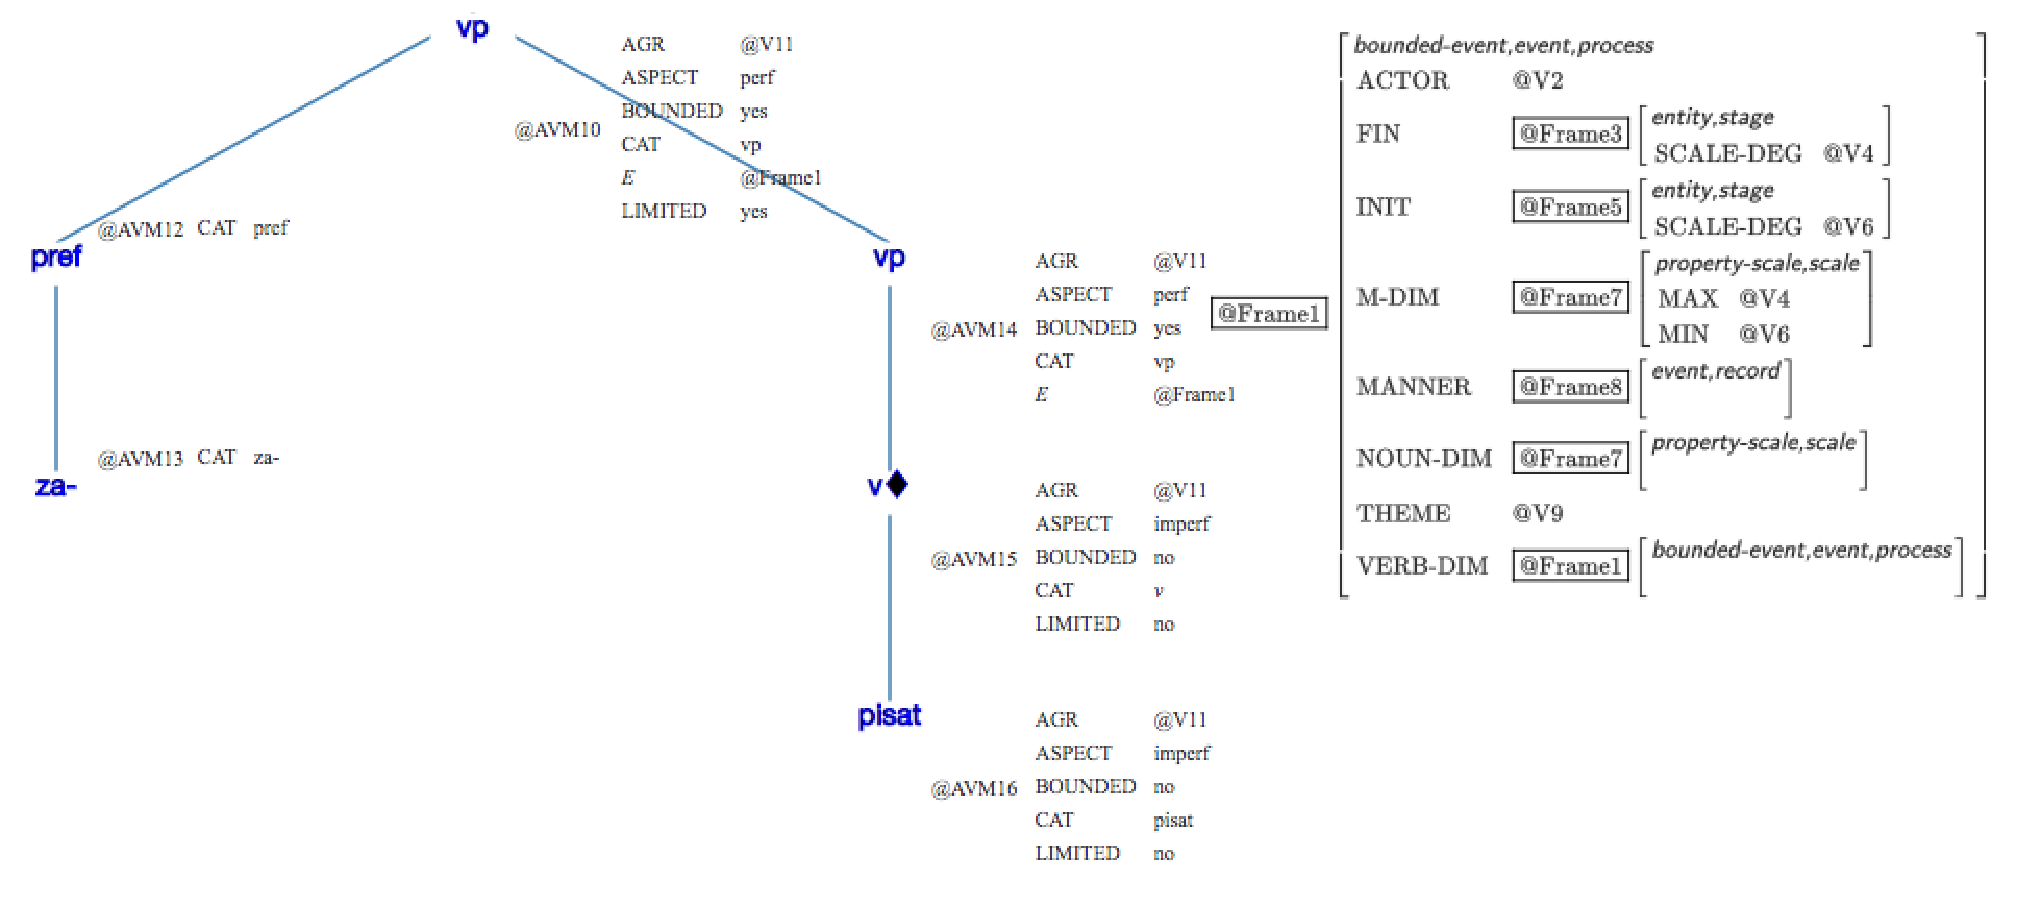
\includegraphics[width=\textwidth]{Zapisat.pdf}
\caption{Result of the compilation of the class \texttt{Zapisat}\label{fig:zapisat}}
\end{sidewaysfigure}

\section{Prefixes}
As we have already discussed the frames for all individual prefix usages in the previous chapter, I will not go through the code for all of them (it can be found in Appendix~\ref{AppendixB}), but show how frames correspond to the \isi{XMG} descriptions and what happens on the syntactic side, taking one prefix as an example.

Figure \ref{code:po} shows the \isi{XMG} description of the class for the prefix \Prefix{po-}. In this code, the syntactic part represents a VP that consists of a prefix head and another (\isi{internal}) VP that carries information about the \isi{derivational base}. The agreement information as well as the semantic frame are then passed to the higher VP node. This node is also characterised by having perfective aspect (one may not call this aspect and consider aspect appearing at a later stage, but then this feature stores the value that will appear as soon as the aspect feature is initialised) independently of the value of the aspect feature of the \isi{internal} VP node. Following the definitions provided above, the feature \textit{limited} is assigned the value \textit{yes} because the semantic frame contains the attribute \FIN, but the feature \textit{bounded} is assigned the value \textit{no}, as the value of the attribute \FIN is a free variable.

\begin{figure}
\begin{lstlisting}[style=xmg]
class PoVerb
export ?VP ?VPInt
declare ?VP ?VPInt ?Po ?PoLex ?AGR ?X0 ?Init ?Fin ?VDim
{
  <syn>{
    node ?VP [cat=vp, agr=?AGR, e=?X0, limited = yes, bounded = no, 
    				 aspect = perf];
    node ?Po [cat=pref];
    node ?PoLex (mark=flex) [cat=po-];
    node ?VPInt [cat=vp, agr=?AGR, e=?X0, bounded = no];
    ?VP -> ?VPInt;
    ?VP -> ?Po;
    ?Po -> ?PoLex;
    ?Po >> ?VPInt
  } ;
  <frame>{
    ?X0[bounded-event,
       m-dim: ?VDim,
       verb-dim: ?VDim,
       init: [stage, 
          scale-deg:?Init],
       fin: [stage, 
          scale-deg:?Fin]    
    ]
  }
}
\end{lstlisting}
\caption{XMG code for the class describing the `delimitative' usage of the prefix \Prefix{po-}\label{code:po}}
\end{figure}

As for the frame description part, it follows straightforwardly earlier proposed frame configuration. To illustrate this, let us compare the code with \figref{frame:po:delim:rep} that shows the frame that was proposed in Chapter~\ref{Chapter7} for the \isi{delimitative} usage of the prefix \Prefix{po-}. If one has a look on those two pictures, it becomes obvious that they differ only with respect to the variable names. 

\begin{figure}
\avm{
\btag{e} [\type*{bounded-event}
   	   \VERBDIM & \1\\
       \MDIM & \1 [\type{scale}] \\
       \INIT & [\type*{stage}
     		\POS & \2]\\
       \FIN & [\type*{stage} 
  		 	\POS & \3 ]
   ]
}
%% Add requirement that if m-dim = path, path-start = init
\caption{Semantic contribution of \Prefix{po-}\label{frame:po:delim:rep}}
\end{figure}

To make sure that the code not only looks similar to the frame, but also produces the desired result, let me show \figref{fig:poverb} that contains the result of the compilation of the proposed \isi{metagrammar} class.

\begin{sidewaysfigure}
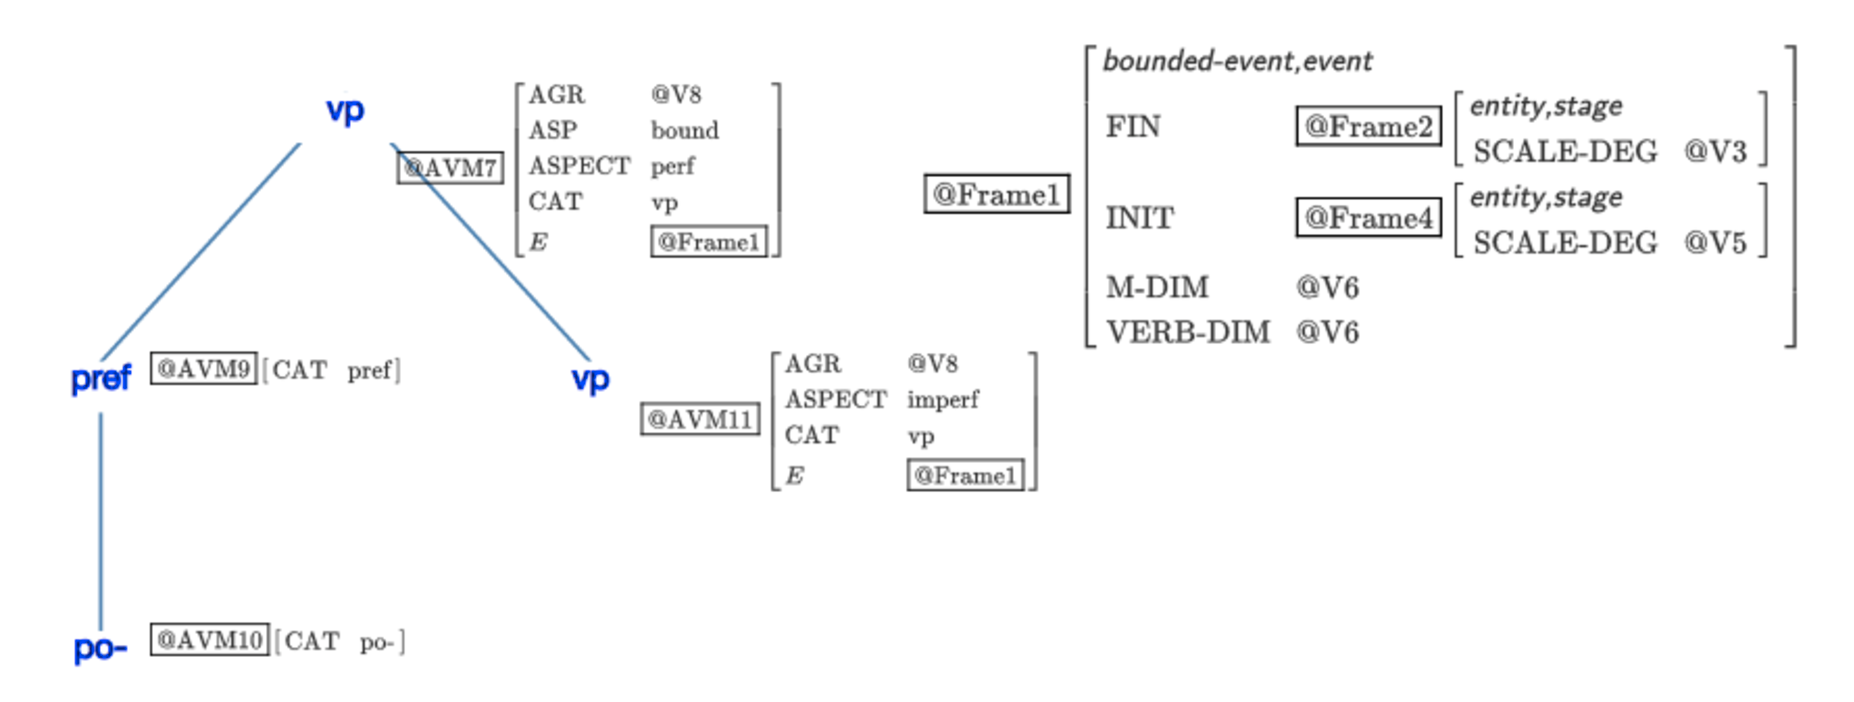
\includegraphics[width=\textwidth]{PoVerb.pdf}
\caption{Result of the compilation of the class \texttt{PoVerb} \label{fig:poverb}}
\end{sidewaysfigure}

%When one contemplates the frame description of the prefix \Prefix{po-} it becomes clear that this prefix rarely can be used in combination with other prefixes or before the attachment of the \isi{secondary imperfective} suffix. If immediately after the attachment of the prefix \Prefix{po-} another prefix is attached, the first step can be just skipped, as it increases the \isi{morphological complexity} and does not influence the resulting semantic representation of the verb. Similar considerations apply if the \Prefix{po-}prefixed verb is to be suffixed with the \isi{imperfective suffix}: normally, the basic \isi{imperfective verbs} would denote the same events as the prefixed and suffixed verb. So even for the presence of some semantic difference, the price of adding two morphemes is too high and such verbs (as \textit{popisyvat'} `to write occasionally, non-seriously') would be used in a restricted number of situations when their meaning is pragmatically enriched. 
%
%If one looks at the situations when the prefix \Prefix{po-} is attached to an already prefixed verb, the picture is also similar: if the last derivation step was \isi{prefixation}, in many cases it has brought at least the semantic information the prefix \Prefix{po-} contains, so further \isi{prefixation} with \Prefix{po-} would be an unnecessary complication. This does not hold for those prefixes that do not overtly add information: e.g., if the verb \textit{zapisat'} `to write down' is suffixed with the suffix \textit{-iva-} in its progressive usage, the resulting verb is defined in terms of being a part of another (bounded) event, but it does not have its own boundaries. The prefix \Prefix{pere-} cannot add such boundaries, as it just copies information, so the verb \textit{perezapisyvat'} `to be rewriting' is imperfective and lacks boundaries, so they will be added when the prefix \Prefix{po-} is attached. Similarly can be explained why the verb \textit{popriotkryt'} `to open very slightly' exists while in other cases an attachment of the prefix \Prefix{po-} to a perfective verb does not seem to be possible (compare with an non-existent verb \textit{*pootkryt'}). In total, the predictions of a semantic-pragmatic analysis in many cases coincide with a syntactic restriction (for \citealt{Tatevosov:13} the prefix \Prefix{po-} is one of the \isi{selectionally limited prefixes}, so it can attach only to \isi{imperfective verbs}) and for some fragments such syntactic restriction may be a fast way of limiting the number of derivation. As we see, however, the analysis proposed here allows for more accurate predictions in complicated cases.
%
%The \isi{distributive} interpretation of the prefix \Prefix{po-} is acquired when the \isi{measure dimension} is the \isi{cardinality scale}. 

Encoding of other prefix usages proceeds in the similar way: the syntactic part does not vary much from prefix to prefix and semantic descriptions can be directly obtained from the frame descriptions I have proposed in Chapter~\ref{Chapter7}. However, there are a couple of difficulties I want to discuss. First let us consider the prefix \Prefix{pere-} in the \isi{repetitive} usage. There are several things that are different compared to the case of the ``\isi{delimitative}'' usage of the prefix \Prefix{po-}. First, the value of the features \textit{aspect} and \textit{bounded} is inherited from the  lower VP and the value of the \textit{limited} feature of the \isi{derivational base} has to be \textit{yes}. Second, at the moment of prefix attachment the central node of the frame shifts: derived VP (node \texttt{?VP} on \figref{code:pere}) is related to the frame \texttt{?X1} whereas the semantics of the \isi{derivational base} is represented by the frame \texttt{?X0} (subframe of \texttt{?X1} on \figref{code:pere}). This realises the solution proposed in the previous chapter. 

\begin{figure}
\begin{lstlisting}[style=xmg]
class PereIterVerb
export ?VP ?VPInt 
declare ?VP ?VPInt ?Pere ?PereLex ?AGR ?X0 ?X1 ?Deg1 ?Deg2 ?Scale ?NounDim
?Aspect ?EventType ?Init ?Fin ?Asp
{
  <syn>{
    node ?VP [cat=vp, agr=?AGR, e=?X1, bounded = ?Asp, limited = yes, 
    				 aspect = ?Aspect];
    node ?Pere [cat=pref];
    node ?PereLex (mark=flex) [cat=pere-];
    node ?VPInt [cat=vp, agr=?AGR, e=?X0, bounded = ?Asp, limited = yes, 
    					  aspect = ?Aspect];
    ?VP -> ?VPInt;
    ?VP -> ?Pere;
    ?Pere -> ?PereLex;
    ?Pere >> ?VPInt
  };
  <frame>{
    ?X1[?EventType,
       m-dim:?Scale[property-scale],
       noun-dim:?NounDim,
       init: ?Init,
       fin: ?Fin,
       prep:?X0[?EventType,
          m-dim:?Scale,
          noun-dim:?NounDim,
          init: ?Init,
          fin: ?Fin]
    ]
  }
}
\end{lstlisting}
\caption{XMG code for the class that describes the repetitive usage of the prefix \Prefix{pere-}\label{code:pere}}
\end{figure}

In order to perform the coercion that is needed when the prefix \Prefix{pere-} is attached to a simplex imperfective verb, a separate step is required. It is realised by the class \texttt{NDimCoercedVerb} (see \figref{xmg:coersion}) that transforms a non-bounded event into a bounded event using the nominal scale.

\begin{figure}
\begin{lstlisting}[style=xmg]
class NDimCoercedVerb
export ?VP ?VPInt
declare ?VP ?AGR ?X0 ?ScMin ?ScMax ?NounDim ?VPInt
{
  <syn>{
    node ?VP [cat=vp, agr=?AGR, e=?X0, bounded = yes, limited = yes, 
    				 aspect = perf];
    node ?VPInt [cat=vp, agr=?AGR, e=?X0, limited = no, aspect = imperf];
    ?VP -> ?VPInt
  };
  <frame>{
    ?X0[bounded-event,
       m-dim: ?NounDim[property-scale & closed-scale,
          min: ?ScMin,
          max: ?ScMax],
       noun-dim:?NounDim,
       init:[stage, 
          scale-deg:?ScMin],
       fin:[stage, 
          scale-deg:?ScMax]
    ]
  }
}
\end{lstlisting}
\caption{XMG code for the class that implements coersion of an unbounded event into a bounded event\label{xmg:coersion}}
\end{figure}

\section{Imperfective suffix}
I use two separate classes to produce two interpretations of \isi{secondary imperfective} verbs: progressive and habitual. For the analysis I propose it is important to distinguish between them when another prefix is attached after the \isi{suffixation}, as these two interpretations have different semantic properties.

The habitual interpretation of the \isi{imperfective suffix}, realised by the code shown on \figref{xmg:habitual}, produces an unlimited event that is a \isi{series of} limited events. The \NOUNDIM of the new event necessarily is of type \textit{cardinality} and does not need to correspond to the respective attribute of the \isi{derivational base}. The \isi{verbal dimension} is copied from the individual event level to the series level. This interpretation of the \isi{imperfective suffix} is also associated with the introduction of the \textit{iteration} type of the event and the respective syntactic feature. The result of the compilation of this class is shown on \figref{fig:iter}.

\begin{figure}
\begin{lstlisting}[style=xmg]
class IterVerb
export ?VP ?VPInt
declare ?VP ?VPInt ?Suf ?Iva ?AGR ?X0 ?X1 ?VDim
{
  <syn>{
    node ?VP [cat=vp, agr=?AGR, e=?X1, bounded = no, limited = no, 
    				  aspect = imperf, iteration = yes];
    node ?Suf [cat=suf];
    node ?Iva (mark=flex) [cat=iva-];
    node ?VPInt [cat=vp, agr=?AGR, e=?X0, limited = yes];
    ?VP -> ?VPInt;
    ?VP -> ?Suf;
    ?Suf -> ?Iva;
    ?VPInt >> ?Suf
  };
  <frame>{
    ?X1[event & iteration,
       segment:?X0[bounded-event,
         noun-dim:[property-scale],
         verb-dim: ?VDim],
       verb-dim: ?VDim,
       noun-dim:[cardinality] 
     ]
  }
}
\end{lstlisting}
\caption{XMG code for the habitual interpretation of the imperfective suffix \label{xmg:habitual}}
\end{figure}

\begin{sidewaysfigure}
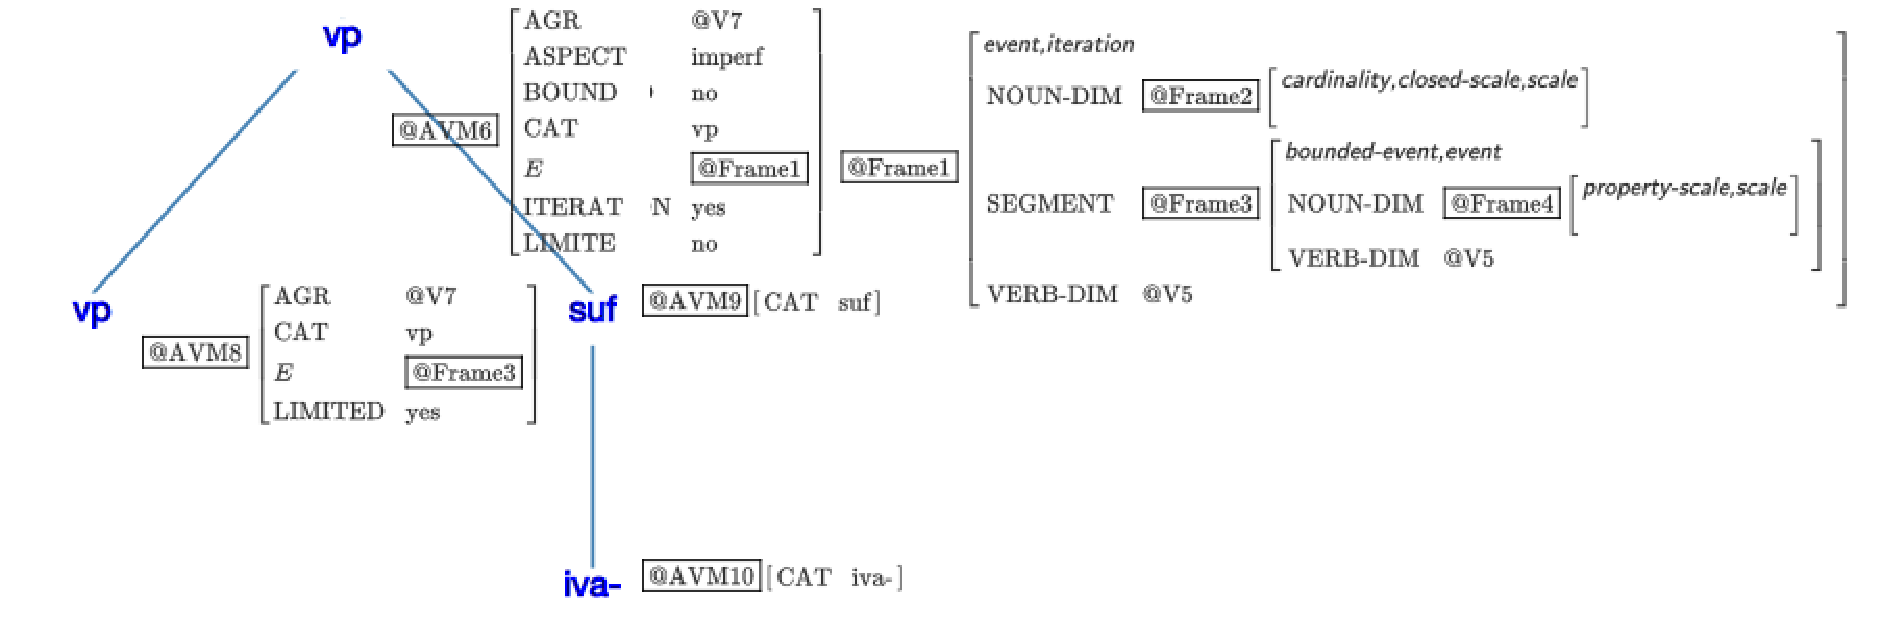
\includegraphics[width=\textwidth]{IterImp.pdf}
\caption{Result of the compilation of the class \texttt{IterVerb}\label{fig:iter}}
\end{sidewaysfigure}

The second interpretation of the \isi{imperfective suffix} is progressive: on the semantic side I represent it as a creation of a new event that is a \PARTOF the event denoted by the \isi{derivational base}. Due to the \PARTOF relation the new event remains limited. On Figures~\ref{graph:pf} and~\ref{graph:ipf} in Chapter~\ref{Chapter1} I have realised \textit{part of} as a relation, as in this case (in contrast to the prefix \Prefix{do-}) it is not functional. As relations are currently not implemented in \isi{XMG}, for the sake of the implementation I use \PARTOF as an attribute when representing the \isi{progressive interpretation} of the \isi{imperfective suffix}.

\section{Assembling the parts}
The last part of the code assembles the verbal phrases from the components described above. As the resource has to be finite, recursion is not allowed in the \isi{XMG} class descriptions.  Due to this restriction, it is not possible to define a single class that would allow an arbitrary number of prefixes to be stacked (by the possibility of attaching a new prefix to the output of the same class). This means that each \isi{prefixation} level has to be described separately. First three classes do the job of assembling verbs with one prefix: the first class (\texttt{OneBasePrefixedVerb}) combines a simplex verb and one of the prefixes; the second class (\texttt{OneCoercedPrefix\-edVerb}) combines a coerced verb with one of the prefixes \Prefix{pere-} (\isi{repetitive} interpretation) and \Prefix{do-}; the last class (\texttt{VerbWithOnePrefix}) assembles under one name the results of the first two classes and all prefixed verbs that are stored in the dictionary. 

\begin{figure}
\begin{lstlisting}[style=xmg]
class TwoPrefixedVerb
export ?VP ?VPInt ?VPBase
declare ?VP ?VPpref ?V ?VSp ?VPInt ?VP ?VPBase
{
  {?VPpref = DoVerb[] | ?VPpref = PereVerb[] | ?VPpref = PereIterVerb[] 
   | ?VPpref = PoVerb[]};
  ?VP = ?VPpref.?VP;
  ?VSp = VerbWithOnePrefix[];
  ?VPInt = ?VSp.?VP;
  ?VPInt = ?VPpref.?VPInt;
  ?VPBase = ?VSp.?VPBase
}
\end{lstlisting}
\caption{XMG code for the verbs with two prefixes \label{xmg:2pref}}
\end{figure}

On the next step (class \texttt{TwoPrefixedVerb}, shown on \figref{xmg:2pref}) the resulting models of the first part are combined again with all available prefix descriptions. This piece of code illustrates how class descriptions are reused: the variable \texttt{?VPpref} gets identified with one of the prefix classes (\texttt{DoVerb}, \texttt{PereVerb}, \texttt{PereIterVerb}, or \texttt{PoVerb}). This is possible only in case all the disjoint classes export the same set of variables. Due to such requirement it is possible to access the exported variables: for example, a \texttt{?VP} variable gets identified with the \texttt{?VP} variable of the \texttt{?VPpref} class (\texttt{?VPpref.?VP}). Similarly the variable \texttt{?VSp} gets identified with a \texttt{VerbWithOnePrefix} class (which, in turn, contains all possible models of verbs with one prefix) and the \texttt{?VPInt} variable is then linked to both the \texttt{?VPInt} node of the \texttt{?VPpref} class and the \texttt{?VP} node of the \texttt{?VSp} class. 

Both types of verbs (with one prefix, \texttt{VerbWithOnePrefix} class, and with two prefixes, \texttt{TwoPrefixedVerb} class) then serve as an input to the class \texttt{SuffVerb}. This class uses the results of \isi{nominal dimension} constructors, as the dimension of the noun can be changed after the attachment of the suffix and it still has to agree with the requirements of the previously attached prefixes. The exported variable \texttt{VPBase} is used to keep track of the attachment point of the semantic representation of the noun. On the syntactic level the noun stays to the right of the verb and will be always attached higher than all the verbal morphemes. 

After the suffixed verbs are assembled, the type matching has to be performed. In the current version of \isi{XMG} type copying is performed not via creating a connection between two types (as it is done with attributes), but by copying the value that is there at the moment the operation is performed. As the noun is attached later, the type of the scale it is associated with is not passed to the higher level if the central node of the frame shifts. To ensure correct typing, I have introduced a class \texttt{TypeMatcher} (code shown on \figref{xmg:typemather}) that identifies all types of the measure dimensions between the higher and the embedded frames (\MDIM, \NOUNDIM, \VERBDIM). The class \texttt{SuffTyped} uses the \texttt{TypeMatcher} class together with the \texttt{SuffVerb} class. In sum, as the VP that contains the scalar interpretation of the noun is identified with the lowest VP available, the type matching mechanism allows to pass the types to a higher level. If the central node of the frame was not changed in the course of prefix attachments, variables \texttt{?X1} and \texttt{?X0} refer to the same frame node.

\begin{figure}
\begin{lstlisting}[style=xmg]
class TypeMatcher
export ?VPOut ?VPInt
declare ?VPInt ?X0 ?X1 ?NDimType ?VDimType ?MDim ?VPOut
{
<syn>{
    node ?VPOut [e=?X1];
    node ?VPInt [e=?X0]
    };
  <frame>{
    ?X1[event,
       m-dim: [?MDim],
       noun-dim: [?NDimType],
       verb-dim: [?VDimType]
    ];
    ?X0[event,
       m-dim: [?MDim],
       noun-dim: [?NDimType],
       verb-dim: [?VDimType]
     ]
  }
}
\end{lstlisting}
\caption{XMG code for the operation of type matching \label{xmg:typemather}}
\end{figure}

I allow for one more derivational step in the described fragment: attachment of a prefix after \isi{suffixation}. This is performed by the class \texttt{TwoPrefixedSuffixedVerb} that uses the result of the compilation of the \texttt{SuffTyped} class and all available prefix classes. At this moment all possible verbal models are created. Then the next step of combining those models with various interpretations of the direct object is performed.

This step is done by two classes: \texttt{PrefixedVerbDirObj} and \texttt{PrefixedSuffixedVerbDirObj} that take, respectively, prefixed and prefixed-suffixed verbs, and all available \isi{dimension constructors}. An output of those classes are models of all possible VPs that use all the available scalar interpretations of the direct objects. This output is again combine with the \texttt{TypeMatcher} class to ensure proper type inheritance.

Before discussing the produced output I would like to note that the architecture of the program is such that as soon as there is a TAG parser that is compatible with frame semantic representation, \isi{lexical anchors} can be removed and the rest of the code would produce unanchored trees with prefixed verbs and appropriate dimension constraints on the argument slot.

%\section{Dimension constructors}
%For the piece I present I need two \isi{dimension constructors}: one referring to the length of the story and another to the cardinality of the set of stories. Both constructors are based on the attributes that are present in the object description: e.g., if there is no \textit{length} attribute in the object frame, the maximum value of the \isi{measure dimension} will be undefined. This is controlled by selecting only appropriate nouns (with a relevant attribute) as those that can undergo the enrichment procedure. Again, as I have to delegate all work to the \isi{metagrammar} compiler, I have to describe such restrictions in the \isi{metagrammar} (see the first line in the class specification), but normally they would be realised as separate \isi{metagrammar} classes and elementary trees for nouns would be accompanied with the information about the possibility of being inserted as \isi{lexical anchors} in such classes.
%
%\begin{figure}
%\begin{lstlisting}[style=xmg]
%%%Creating appropriate dimensions for objects
%
%class NounLength
%export ?N
%declare ?NLength ?X0 ?Length ?N
%{
%  ?NLength=Story[];
%  ?NLength.?Length = ?Length;
%  ?N=?NLength.?N;
%  <syn>{
%    node ?N (mark=coanchor)[cat=n, i=?X0]
%  };
%  <frame>{
%   ?X0[entity,
%        m-dim:[length,
%            min:[zero],
%            max:?Length
%            ]
%      ]
%  }
%}
%
%%% Plural nouns can be interpreted as introducing a \isi{cardinality scale}
%class NounCardinal
%export ?N
%declare ?NCard ?X0 ?Card ?N
%{
%  ?NCard=Story[];
%  ?NCard.?Card = ?Card;
%  ?N=?NCard.?N;
%  <syn>{
%    node ?N (mark=coanchor)[cat=n, num = pl, i=?X0]
%  };
%  <frame>{
%   ?X0[entity,
%        m-dim:[cardinality,
%            min:[zero],
%            max:?Card
%            ]
%      ]
%  }
%}
%\end{lstlisting}
%\caption{Nominal dimension constructors: length and cardinality}
%\end{figure}
%
%After all the constructors are applied, in my implementation they are assembled in one class called \texttt{NDim}. This class creates a VP head and information about \THEME gets included into the newly created event frame. Information about the dimension of the noun is copied to the \NOUNDIM attribute of the event. Note that the case is not specified: this is done in order to account for the possibility of genitive objects and expresses the idea that it is the verb that governs the case assignment and the semantic operation of dimension construction is related but not always governed by the morphological form of the noun. 
%
%\begin{figure}
%\begin{lstlisting}[style=xmg]
%class NDim
%export ?NP ?N ?VP
%declare ?VP ?NP ?X0 ?Theme ?Dim ?Case ?N ?Noun ?Num
%{
%  {?Noun=NounCardinal[] | ?C=NounLength[]};
%  ?N=?Noun.?N;
%  <syn>{
%    node ?NP [cat=np, case=?Case, num = ?Num, i=?Theme];
%    node ?VP [cat=vp, e=?X0];
%    node ?N (mark=coanchor) [cat=n, case = ?Case, num = ?Num, i=?Theme];
%    ?VP >>+ ?NP;
%    ?NP -> ?N
%  }  
%  ;
%  <frame>{
%    ?X0[event,
%          theme:?Theme[entity,
%	          m-dim:?Dim
%          ],
%      noun-dim:?Dim      
%    ]
%  }
%}
%\end{lstlisting}
%\end{figure}

\section{Output}\largerpage
The compilation of the code produces 88 verbal phrases. The full xml of the output is provided in Section~\ref{B:Tat} of Appendix~\ref{AppendixB}. Here I will show and provide a brief analysis of all the obtained models.

The first group of models consists of verbs with one or two prefixes. A total of 16 models is produced (see Table~\ref{table:prefverbs}). Six of these models are models of verbs with one prefix. They all exist, but this is partially due to the selection of the prefixes and the base verb. The upper part of Table~\ref{table:prefverbs} shows these verbs with their English translations and the dimension interpretation of the argument. The last two columns indicate whether the verb exists and if not, whether it will be filtered out by pragmatic module as described in Chapter~\ref{Chapter6}.\largerpage

\begin{table}
\caption{Output of the XMG processing for the class of one- or two-prefixed verbs\label{table:prefverbs}}
\resizebox{\textwidth}{!}{\begin{tabular}{lllll}
\lsptoprule
verb  & semantics & noun  & exists  & blocked by \\
      &           & interpretation & &    pragmatics \\     \midrule
popisat' & to write for some time & length & yes & -- \\ 
dopisat' & to finish writing & length & yes & -- \\ 
perepisat' & to rewrite & length & yes  & --\\ 
zapisat' & to write down & length & yes  & --\\ 
perepisat' & to write all of & cardinal & yes  & --\\ 
popisat' & to write all of & cardinal & yes  & --\\\midrule
dodopisat' & to finish finishing writing & length & yes & -- \\ 
doperepisat' & to finish rewriting & length & yes & -- \\ 
dozapisat' & to finish writing down & length & yes & -- \\ 
peredopisat' & to refinish writing & length & yes & -- \\ 
pereperepisat' & to rewrite again & length & yes  & --\\ 
perezapisat' & to write down again & length & yes & -- \\ 
popopisat' & to write for some time & length & no & yes \\  
perepopisat' & to write all of & cardinal & no & yes \\  
popopisat' & to write all of & cardinal & no & yes \\ 
doperepisat' & to finish writing all of & cardinal & yes & -- \\ 
\lspbottomrule
\end{tabular}}
\end{table}

In the second part of \tabref{table:prefverbs} verbs that contain two prefixes are present. Out of those verbs three must be filtered out for pragmatic reasons since their semantics is equivalent to the semantics of simpler verbs: two variant of the verb \textit{popopisat'} are associated with exactly the same frames as two variants of the verb \textit{popisat'} `to write for some time/to write all of' that can be found in the upper part of the Table~\ref{table:prefverbs}. The third verb that also needs to be discarded is the verb \textit{perepopisat'} that has exactly the same representation as the verb \textit{perepisat'}`to write all of'. 

Note that already at this stage \isi{XMG} reduces 40 possible models (five variants of the first prefix, four variants of the second prefix, and two interpretations of the noun) to only 10 (seven correct and three non-existent) by an appropriate combination of constraints. 

Now let us have a look at the next step: when the verbs from the list above get suffixed with the \isi{imperfective suffix} (in one of two interpretations). The output of this part consists of 23 verbs out of which only two must be filtered out as they are produced on the basis of the verbs that, as we have discussed above, do not exist: \textit{perepopisat'} `to write all of' and \textit{popopisat'} `to write for some time'. It is interesting to note that the second interpretation of the last verb does not get suffixed, so the number of wrong models on the new level does not get multiplied (by the two possible interpretations of the suffix). Instead of the six potential incorrect models just on the basis of the wrong predictions of the previous level we obtain only two. All the verbs produced by this part of the implementation are shown in Table~\ref{table:suffverbs} together with their English translations, interpretation of the \isi{imperfective suffix}, and information about existence.\largerpage

\begin{table}
 \caption{Output of the XMG processing for the class of prefixed and then suffixed verbs\label{table:suffverbs}}
\resizebox{\textwidth}{!}{\begin{tabular}{llll}
\lsptoprule
verb  & semantics & imperfective & exists \\ 
      &      &    interpretation\\\midrule
perepisyvat' & to be writing all of & progressive & yes\\ 
popisyvat' & to be writing for some time habitually & habitual & yes \\ 
dopisyvat' & to be finishing writing & progressive & yes \\ 
dopisyvat' & to finish writing habitually & habitual & yes \\ 
perepisyvat' & to be rewriting & progressive & yes \\ 
perepisyvat' & to rewrite habitually & habitual & yes \\ 
zapisyvat' & to be writing down & progressive & yes \\ 
zapisyvat' & to write down habitually & habitual & yes \\ 
doperepisyvat' & to be finishing writing all of & progressive & yes\\ 
dodopisyvat' & to be finishing writing the final part & progressive & yes \\ 
dodopisyvat' & to finish writing the final part habitually & habitual & yes \\ 
doperepisyvat' & to be finishing rewriting & progressive & yes \\ 
doperepisyvat' & to finish rewriting habitually & habitual & yes \\ 
dozapisyvat' & to be finishing writing down & progressive & yes \\ 
dozapisyvat' & to finish writing down habitually & habitual & yes \\ 
perepopisyvat' & to be writing all of & progressive & no\\ 
peredopisyvat' & to be rewriting the final part & progressive & yes \\ 
peredopisyvat' & to rewrite the final part habitually & habitual & yes \\ 
pereperepisyvat' & to be rewriting again & progressive & yes \\ 
pereperepisyvat' & to rewrite again habitually & habitual & yes \\ 
perezapisyvat' & to be writing down again & progressive & yes \\ 
perezapisyvat' & to write down again habitually & habitual & yes \\ 
popopisyvat' & to be writing for some time habitually & habitual & no\\ 
 \lspbottomrule
 \end{tabular}}
\end{table}

The last group of verbs consists of 49 models that contain at least one prefix attached before the \isi{imperfective suffix} and at least one prefix attached after it. They are shown in Table~\ref{table:prefsuffverbs} together with English translations (not always exact) and the aspect (as here some of the verbs, despite being prefixed on the last derivation step, are imperfective). This part is harder to evaluate as many of the verbs cannot be found on the internet. A possible evaluation method would be to test the unanchored models with various \isi{lexical anchors} against corpus data, but this requires both the parser that supports \isi{frame semantics} (to work efficiently with different verbs) and a large corpus that contains \isi{complex verbs}. I leave these tasks for future research.\largerpage[-1]
 
\begin{longtable}{lll}
\caption{Output of the XMG processing for the class of verbs that are prefixed, then possibly suffixed, and then prefixed again \label{table:prefsuffverbs}}\\
\lsptoprule verb  & semantics & aspect\\ \midrule\endfirsthead%
\midrule verb  & semantics & aspect\\ \midrule\endhead\endfoot\lspbottomrule\endlastfoot
*perepopisyvat' & -- & perfective \\ 
peredopisyvat' & to write the final parts of all of & perfective \\ 
pereperepisyvat' & co copy/rewrite all of & perfective \\ 
perezapisyvat' & to write down all of & perfective \\ 
peredodopisyvat' & to write the very final parts of all of & perfective \\ 
peredoperepisyvat' & to finish rewriting all of & perfective \\ 
peredozapisyvat' & to finish writing down all of & perfective \\ 
pereperedopisyvat' & to rewrite the final parts all of & perfective \\ 
perepereperepisyvat' & co copy/rewrite again all of & perfective \\ 
pereperezapisyvat' & to write down again all of & perfective \\ 
*perepopopisyvat' & \isi{derivational base} does not exist & perfective \\\midrule

*popopisyvat' & to write for some time habitually all of & perfective \\ 
podopisyvat' & to finish writing all of & perfective \\ 
poperepisyvat' & to rewrite all of & perfective \\ 
pozapisyvat' & to write down all of & perfective \\ 
pododopisyvat' & to write the very final parts of all of  & perfective \\ 
podoperepisyvat' & to finish rewriting all of  & perfective \\ 
podozapisyvat' & to finish writing down all of  & perfective \\ 
poperedopisyvat' & to rewrite the final part all of  & perfective \\ 
popereperepisyvat' & co copy/rewrite again all of  & perfective \\ 
poperezapisyvat' & to write down again all of & perfective \\  
*popopopisyvat' & \isi{derivational base} does not exist & perfective\\  \midrule

dodopisyvat' & to finish writing the final part & perfective \\ 
doperepisyvat' & to finish rewriting & perfective \\ 
dozapisyvat' & to finish writing down & perfective \\ 
dododopisyvat' & to finish writing the very final part & perfective \\ 
dodoperepisyvat' & to finish the final part of rewriting   & perfective \\ 
dodozapisyvat' & to finish writing down the final part  & perfective \\ 
doperedopisyvat' & to finish rewriting the final part  & perfective \\ 
dopereperepisyvat' & to finish rewriting again & perfective \\ 
doperezapisyvat' & to finish writing down again & perfective \\  \midrule

peredopisyvat' & to be rewriting the final part & imperf \\ 
pereperepisyvat' & to be rewriting again & imperf\\ 
perezapisyvat' & to be writing down again & imperf\\ 
peredodopisyvat' & to be finishing rewriting the final part & imperf\\ 
peredoperepisyvat' & to be finishing rewriting  again & imperf\\ 
peredozapisyvat' & to be writing down the final part again & imperf \\ 
pereperedopisyvat' & to be rewriting the final part again & imperf \\ 
perepereperepisyvat' & to be rewriting for the forth time & imperf \\ 
pereperezapisyvat' & to be writing down for the third time & imperf \\  \midrule

podopisyvat' & to spend some time finishing writing & perfective \\ 
poperepisyvat' & to spend some time rewriting & perfective \\ 
pozapisyvat' & to spend some time writing down & perfective \\ 
pododopisyvat' & to spend some time finishing the final part & perfective \\ 
podoperepisyvat' & to spend some time finishing rewriting & perfective \\ 
podozapisyvat' & to spend some time finishing writing down & perfective \\ 
poperedopisyvat' & to spend some time rewriting the final part & perfective \\ 
popereperepisyvat' & to spend some time rewriting again & perfective \\ 
poperezapisyvat' & to spend some time writing down again & perfective \\  
\end{longtable}

\pagebreak According to the available data and introspection, out of 49 models four must be discarded. Two of them (\textit{popopopisyvat'} and \textit{perepopopisyvat'}) are formed from the derivational bases that need to be discarded (discussed above). Other two must be discarded by the pragmatic module.

The first of the two verbs, \textit{*perepopisyvat'}, that could have been translated as `to write all of for some time' would be blocked because the interpretation of the prefix \Prefix{pere-} related with the \isi{cardinality scale} is `performing the action completely with each item in the set'. Now, if the interpretation of the prefix \Prefix{po-} does not get strengthened (some time $\rightarrow$ all context-specified time), we obtain a contradiction.  If it does get strengthened (every writing event is maximal with respect to the corresponding member of the set), then the same semantics can be expressed by the simpler verb \textit{perepisat'} `to write all of'. 

The second verb, \textit{*popopisyvat'}, has a similar semantic structure and also could be translated as `to write all of for some time' (see the discussion about the differences between the \isi{distributive} interpretations of the prefixes \Prefix{po-} and \Prefix{pere-} in Chapter~\ref{Chapter5}). This verb refers to the same set of events as the verb \textit{popisat'} with \isi{distributive} interpretation (`to write all of'), although the surface semantic representations of the two verbs are different, so a deeper analysis is needed in this case.

By now we have seen all the models that my implementation produces. Out of 88 models nine should be discarded, but what is harder to evaluate is the recall of the model (fraction of the number of correct models in the output to the number of correct models), as there is no standard that would provide the later number (the total of correct models for the described grammar fragment). I will approach this problem in the next section.

\section{Result evaluation and comparison}
In order to compare the predictions of my model to that of earlier theories, I have implemented the system proposed in \citet{Tatevosov:09} for exactly the same fragment (one verbal stem, one ``lexical'' prefix, five prefix-interpretation pairs, the \isi{imperfective suffix}). For this part I have omitted the lexical entries for direct objects as they do not influence the interpretation of the prefixed verbs. As the approach is syntactic, all restrictions are formulated in syntactic terms and the frame dimension is used to represent the order of attachment of affixes with different semantics. In this implementation, for example, the class for the \isi{distributive} interpretation of the prefix \Prefix{pere-} looks as shown on \figref{xmg:Tat:pere}. The restriction on this prefix attachment is the imperfective aspect of the base verb, which is reflected via a syntactic constraint on the feature \textit{aspect} here.

\begin{figure}
\begin{lstlisting}[style=xmg]
class PereVerb
export ?VP ?VPInt 
declare ?VP ?VPInt ?Pere ?PereLex ?AGR ?X0 ?X1 
{
  <syn>{
    node ?VP [cat=vp, agr=?AGR, e=?X1, aspect = perf];
    node ?Pere [cat=pref];
    node ?PereLex (mark=flex) [cat=pere-];
    node ?VPInt [cat=vp, agr=?AGR, e=?X0, aspect = imperf];
    ?VP -> ?VPInt;
    ?VP -> ?Pere;
    ?Pere -> ?PereLex;
    ?Pere >> ?VPInt
  };
  <frame>{
    ?X1[distributive,
       of: ?X0]
  }
}
\end{lstlisting}
\caption{XMG implementation for the distributive interpretation of the prefix \Prefix{pere-} according to the theory of \citet{Tatevosov:09}\label{xmg:Tat:pere}}
\end{figure}

However, a direct \isi{comparison} of the predictions of the two models is not possible, as \citet{Tatevosov:09} does not offer any theory about the nature of various interpretations of the \isi{imperfective suffix}. Two solutions are available in this situation: either introduce both interpretations of the \isi{imperfective suffix} in the implementation of the theory proposed by \citet{Tatevosov:09} or count those models produced with the implementation of my theory that differ only with respect to the interpretation only once. The second option requires more manual checking, but is more fair with respect to the analysis of \citet{Tatevosov:09}, so I decided to adopt it.

My implementation of the analysis proposed in \citet{Tatevosov:09} produces 81 models for the same fragment. I have done a full analysis of the resulting models and I would like to show the results from verbs with two prefixes and the verbs that are prefixed after the \isi{imperfective suffix} is attached. At the end I will provide the summary with precision, recall, and F-score data for the two models.

%\begin{table}
%\begin{tabular}{p{3.0cm} | p{3cm} | c | c | c}
%verb  & semantics & exists & this model  & Tatevosov 09\\
%perepisyvat' & imperf (to write all of) & yes & + & +\\ \hline
%popisyvat' & imperf (to write for some time) & yes & + & +\\ \hline
%dopisyvat' & imperf (to finish writing) & yes & + & +\\ \hline
%perepisyvat' & imperf (to rewrite) & yes & + & + \\ \hline
%zapisyvat' & imperf (to write down) & yes & + & + \\ \hline
%doperepisyvat' & imperf (to finish writing all of) & yes & + & +\\ \hline
%dodopisyvat' & imperf (to finish writing the final part) & yes & + & + \\ \hline
%dopopisyvat' & imperf (to finish writing for some time) & no & - & + \\ \hline
%doperepisyvat' & imperf (to finish rewriting) & yes & + & + \\ \hline
%dozapisyvat' & imperf (to finish writing down) & yes & + & +\\ \hline
%perepopisyvat' & to be writing all of & no & + & - \\ \hline
%peredopisyvat' & imperf (to rewrite the final part) & yes & + & + \\ \hline
%pereperepisyvat' & imperf (to be rewriting all of) & no & - & + \\ \hline
%pereperepisyvat' & imperf (to rewrite again) & yes & + & + \\ \hline
%perepopisyvat' & imperf (to write for some time again) & no & - & + \\ \hline
%perezapisyvat' & imperf (to write down again) & yes & + & + \\ \hline
%popopisyvat' & to be writing occasionally & no & +  & - \\ \hline
% \hline
% \end{tabular}
%\end{table}
% 
%12 correct (both approaches)
%Tatevosov: 3 wrong
%me: 2 wrong

Table~\ref{table:twopref} shows the full list of verbs produced by two implementations. As we have already discussed above, seven verbs in this list exist and the ``semantic'' implementation produces three models that have to be discarded. The model of the analysis by \citet{Tatevosov:09} produces five verbs that do not exist (under the interpretation associated with them) and three verbs that should be discussed in more detail (marked with question marks in the table).

\begin{table}
\caption{Verbs with two prefixes produced by two implementations \label{table:twopref}}
\begin{tabular}{ll c c c}
\lsptoprule
verb  & semantics & exists & this   & \citeauthor{Tatevosov:09}\\
      &           &        &     account           &  (\citeyear{Tatevosov:09})\\\midrule
dodopisat' & to finish finishing writing & yes & + & + \\ 
doperepisat' & to finish rewriting & yes & + & + \\ 
doperepisat' & to finish writing all of & yes & + & + \\ 
dopopisat' & to finish writing for some time & no & \textminus & + \\ 
dozapisat' & to finish writing down & yes & + & + \\ 
peredopisat' & to refinish writing & yes & + & + \\ 
pereperepisat' & to rewrite all of & no & \textminus & +\\ 
pereperepisat' & to rewrite again & yes & +  & +\\ 
perepopisat' & to write for some time again & no & \textminus & + \\  
perezapisat' & to write down again & yes & + & + \\ 
podopisat' & to finish writing all of & ?? & \textminus & + \\  
poperepisat' & to rewrite all of & ?? & \textminus & + \\  
poperepisat' & to write all of & no & \textminus & + \\  
popopisat' & to write all of for some time & no & \textminus & + \\  
pozapisat' & to rewrite all of & ?? & \textminus & + \\  
popopisat' & to write for some time & no & + & \textminus \\  
perepopisat' & to write all of & no & + & \textminus \\  
popopisat' & to write all of & no & + & \textminus \\ 
\lspbottomrule 
\end{tabular}
\end{table}
%7 exist, predicted by both accounts
%5 false + 3 questionable predicted by Tatevosov 
%3 false predicted by the current approach (to be discarded by the pragmatics module)

These three verbs are verbs that contain the \isi{distributive} prefix \Prefix{po-} stacked over some other prefix (with non-\isi{distributive} interpretation): \textit{podopisat'} `to finish writing all of', \textit{poperepisat'} `to rewrite all of', and  \textit{pozapisat'} `to rewrite all of'. They are, according to the theory proposed in \citet{Tatevosov:09}, possible, but not extensively discussed in the paper (a manuscript by the same author, dedicated to this usage of the prefix and cited among the references, never appeared). I personally do not find them acceptable and \citet[143]{Tatevosov:09} himself marks such verbs as ``interpretable with difficulty''. They could be accommodated in my account if the \isi{distributive} interpretation of the prefix \Prefix{po-} is represented separately and is two-layered, effectively combining in itself the semantics of the \isi{imperfective suffix} (iterative/habitual interpretation) and the current representation of the prefix \Prefix{po-}. The piece of code shown on \figref{xmg:podistr} implements this solution and allows to produce exactly those three verbs (if the class is combined with verbs that are already prefixed once). One would probably want to associate this representation with a higher cost in \isi{comparison} with the initial representation I offer if a subsequent pragmatic module is used.

\begin{figure}
\begin{lstlisting}[style=xmg,basicstyle=\ttfamily\small]
class PoDistrVerb
export ?VP ?VPInt
declare ?VP ?VPInt ?Po ?PoLex ?AGR ?X0 ?X1 ?Init ?Fin ?VDim
{
  <syn>{
    node ?VP [cat=vp, agr=?AGR, e=?X1, limited = yes, bounded = yes, 
    				 aspect = perf, iteration = yes];
    node ?Po [cat=pref];
    node ?PoLex (mark=flex) [cat=po-];
    node ?VPInt [cat=vp, agr=?AGR, e=?X0, bounded = yes];
    ?VP -> ?VPInt;
    ?VP -> ?Po;
    ?Po -> ?PoLex;
    ?Po >> ?VPInt
  };
  <frame>{
    ?X1[bounded-event & iteration,
       m-dim:?VDim[cardinality],
       verb-dim: ?VDim,
       segment:?X0[event,
         m-dim:[property-scale]
       ]
    ]
  }
}
\end{lstlisting}
\caption{XMG code for implementing the `coerced' distributive interpretation of the prefix \Prefix{po-}\label{xmg:podistr}}
\end{figure}

If the three verbs that we have just discussed are considered existent, then the \isi{prefixation} system proposed by \citet{Tatevosov:09} produces five models that must be discarded. In contrast with my proposal, there is no further explanation of why exactly those verbs (two of them are produced by the same rule that forms the three verbs we have just discussed) would be problematic.

Among the verbs with one or two prefixes and an \isi{imperfective suffix} added at the last step of the derivation the number of errors stays close (two versus three), although again constructed but not existent verbs are distinct in two approaches. Both implementations have full recall with respect to this part and the part we have discussed before.

The \isi{comparison} becomes more interesting when  we consider the most \isi{complex verbs} created by the two implementations. The number of models produced here is close: 45 models according to the analysis by \citet{Tatevosov:09} and 49 models in the implementation of my analysis. The overlap of these sets constitutes, however, only 27 models. The first thing to note is that the group of verbs that are marked as imperfective in Table~\ref{table:prefsuffverbs} cannot be (and is not) produced in the system proposed by \citet{Tatevosov:09}. One may ask whether they should be produced at all: an attentive reader probably noticed that both Table~\ref{table:suffverbs} and Table~\ref{table:prefsuffverbs} contain, for example, the imperfective verb \textit{perezapisyvat'} `to be writing down again'. The structure of the two verbs, however, is different: in one case the \isi{imperfective suffix} is attached as the last step of the derivation and in the other case it happens before the \isi{repetitive} \Prefix{pere-} is attached. On the semantic side this is reflected in what ends up to constitute the preparatory stage of the event: once it is the whole completed event of the same type, and in the second case it is another ongoing/partial event. Another difference is that only in the first structure the habitual interpretation of the suffix is possible. 

The second group of \isi{complex verbs} that is not produced by the implementation of the analysis offered in \citealt{Tatevosov:09} is formed by the verbs with the outermost prefix \Prefix{do-}. They follow the pattern we have extensively discussed in Chapter~\ref{Chapter2}.

Among the rest of the models produced by the second implementation are such verbs as \textit{pereperepopisyvat'} with a semantic structure of a \isi{distributive} interpretation over imperfective of the \isi{repetition} of a delimited event. Such semantic structures are hardly conceivable and the corresponding verbs do not exist.\footnote{This judgement is mostly based on introspection and personal communication with other native speakers, as any such verb would be rare and the absence of data on the Internet is not a reliable indicator of the non-existence. I plan to conduct additional experiments in future to get statistically reliable evidence about the existence of such \isi{complex verbs}.}

%\begin{tabular}{p{3cm} | p{6cm} | p{2cm}} 
%verb  & semantics & aspect\\ \hline
%+*perepopisyvat' & -- & perfective \\ \hline
%+peredopisyvat' & to write the final parts of all of & perfective \\ \hline
%pereperepisyvat' & for all: imperf (write all of) & Tatevosov\\
%+pereperepisyvat' & co copy/rewrite all of & perfective \\ \hline
%+perezapisyvat' & to write down all of & perfective \\ \hline
%+peredodopisyvat' & to write the very final parts of all of & perfective \\ \hline
%+peredoperepisyvat' & to finish rewriting all of & perfective \\ \hline
%peredoperepisyvat' & for all: imperf (finish rewriting all of) & Tatevosov \\ \hline
%peredopopisyvat' & distr (imp (compr (delim))) & Tatevosov \\ \hline
%+peredozapisyvat' & to finish writing down all of & perfective \\ \hline
%+pereperedopisyvat' & to rewrite the final parts all of & perfective \\ \hline
%perepereperepisyvat' & co copy/rewrite again all of & perfective \\ \hline
%perepereperepisyvat' & distr (imp (rep (distr))) & Tatevosov \\ \hline
%pereperepopisyvat' & distr (imp (rep (delim))) & Tatevosov \\ \hline
%+pereperezapisyvat' & to write down again all of & perfective \\ \hline
%*perepopopisyvat' & \isi{derivational base} does not exist & perfective \\ \hline  \hline
%
%
%+*popopisyvat' & distr (imp (delim)) & perfective \\ \hline
%+podopisyvat' & to finish writing all of & perfective \\ \hline
%+poperepisyvat' & to rewrite all of & perfective \\ \hline
%poperepisyvat' & distr (imp (distr)) & Tatevosov \\ \hline
%+pozapisyvat' & to write down all of & perfective \\ \hline
%+pododopisyvat' & to write the very final parts of all of  & perfective \\ \hline
%+podoperepisyvat' & to finish rewriting all of  & perfective \\ \hline
%podoperepisyvat' & distr (imp (compl (distr))) & Tatevosov \\ \hline
%podopopisyvat' & distr (imp (compl (delim))) & Tatevosov \\ \hline
%+podozapisyvat' & to finish writing down all of  & perfective \\ \hline
%+poperedopisyvat' & to rewrite the final part all of  & perfective \\ \hline
%+popereperepisyvat' & co copy/rewrite again all of  & perfective \\ \hline
%popereperepisyvat' & distr (imp (rep (distr))) & Tatevosov \\ \hline
%+poperezapisyvat' & to write down again all of & perfective \\ \hline
%poperepopisyvat' & distr (imp (rep (delim))) & Tatevosov \\ \hline
%*popopopisyvat' & \isi{derivational base} does not exist & perfective\\ \hline
%
%dodopisyvat' & to finish writing the final part & perfective \\ \hline
%doperepisyvat' & to finish rewriting & perfective \\ \hline
%dozapisyvat' & to finish writing down & perfective \\ \hline
%dododopisyvat' & to finish writing the very final part & perfective \\ \hline
%dodoperepisyvat' & to finish the final part of rewriting   & perfective \\ \hline
%dodozapisyvat' & to finish writing down the final part  & perfective \\ \hline
%doperedopisyvat' & to finish rewriting the final part  & perfective \\ \hline
%dopereperepisyvat' & co finish rewriting again & perfective \\ \hline
%doperezapisyvat' & to finish writing down again & perfective \\ \hline \hline
%
%peredopisyvat' & to be rewriting  the final part & imperfective \\ \hline
%pereperepisyvat' & to be rewriting again & imperfective\\ \hline
%perezapisyvat' & to be writing down again & imperfective\\ \hline
%peredoperepisyvat' & to be finishing rewriting  again & imperfective\\ \hline
%peredozapisyvat' & to be writing down the final part again & imperfective \\ \hline
%pereperedopisyvat' & to be rewriting the final part again & imperfective \\ \hline
%perepereperepisyvat' & to be rewriting for the forth time & imperfective \\ \hline
%pereperezapisyvat' & to be writing down for the third time & imperfective \\ \hline \hline
%
%+podopisyvat' & to spend some time finishing writing & perfective \\ \hline
%+poperepisyvat' & to spend some time rewriting & perfective \\ \hline
%poperepisyvat' & to spend some time writing all of & Tatevosov \\ \hline
%popopisyvat' & to spend some time writing for some time & Tatevosov \\ \hline
%+pozapisyvat' & to spend some time writing down & perfective \\ \hline
%+pododopisyvat' & to spend some time finishing the final part & perfective \\ \hline
%+podoperepisyvat' & to spend some time finishing rewriting & perfective \\ \hline
%podoperepisyvat' & delim (imp (comp (distr))) & Tatevosov \\ \hline
%podopopisyvat' & delim (imp (comp (delim))) & Tatevosov \\ \hline
%+podozapisyvat' & to spend some time finishing writing down & perfective \\ \hline
%+poperedopisyvat' & to spend some time rewriting the final part & perfective \\ \hline
%+popereperepisyvat' & to spend some time rewriting again & perfective \\ \hline
%popereperepisyvat' & delim (imp (rep (distr))) & Tatevosov \\ \hline
%poperepopisyvat' & delim (imp (rep (delim))) & Tatevosov \\ \hline
%+poperezapisyvat' & to spend some time writing down/copying again & perfective \\ \hline
%\end{tabular}
%\caption{Output of the XMG processing for the class of verbs that are prefixed, then possibly suffixed, and then prefixed again {table:prefsuffverbs}}
%\end{table}

%6+ 7 +3 + 12 + 27 + 18 = 28 + 28 + = 73
%6+10+12+27 = 28+27 = 55
%5+3 +18
%-3 +2+4+3
%So out of 45 models produced for the prefixed, suffixed, and then prefixed again verbs by the implementation of the analysis proposed in \citet{Tatevosov:09} I think that 27 exist, 18 do not, and 18 are missed. 
%
%
%Tatevosov: total 121. Me: total 88. -9 = 79
%Overlap: 51 correct models + 2 incorrect both approaches + 18 correct my approach  + 7 wrong my approach
%+ 25 wrong Tatevosov + 3 questionable Tatevosov + 40 incorrect
%51 - 3 - 67
%51 + 17 + 3 = 71
%+9

To quantify precision and recall, I decided to do the following:
\begin{itemize}
\item count 79 models instead of 88 for my analysis by removing such models that differ only with respect to the interpretation of the \isi{secondary imperfective};
\item count the models for the existence of which I argue in Chapter~\ref{Chapter2} as correct (\isi{imperfective verbs} formed when the last affix attached is the \isi{repetitive} \Prefix{pere-} and perfective \Prefix{do-}prefixed verbs)
\item calculate all measures two times: once counting three questionable verbs as incorrect (Table~\ref{table:precision}) and once counting them as correct (Table~\ref{table:precision2});
\item on pair with the previous decision I will use two versions of the implementation of my analysis: the original one and one that uses the update shown in \figref{xmg:podistr}.
\end{itemize}
 
Based on this, I obtain the following numbers: for the implemented fragment there are 70 or 73 correct models\footnote{I have manually checked the possibilities using the assumption that there can be no existing complex verb derived from a non-existing verb. The calculation of the recall is thus based on this assumption.}. Out of these models, the implementation of the analysis provided in \citet{Tatevosov:09} produces, respectively, 52 or 55, and the total number of models output is 81. The original implementation of my analysis produces 70 correct models and the total number of models (after the duplicates among \isi{imperfective verbs} are removed) is 79. The updated version produces 70 and 73 of the correct models, respectively, and the total number of models in this case is 82. The precision (fraction of correct models out to all produced models), recall (fraction of correct models in the output to all correct models), and F-measures ($2*(precision*recall)/(precision+recall)$) are provided in Table~\ref{table:precision} for the first version of calculation (three questionable models excluded) and in Table~\ref{table:precision2} for the second version.
 
 \begin{table}
 \caption{Precision, recall and F-measure for different implementations (three questionable verbs excluded) \label{table:precision}}
 \begin{tabular}{l *{3}{S[table-format=1.3]}}
 \lsptoprule
 analysis & {precision} & {recall} & {F-measure}\\ \midrule
 current analysis original & 0.886 & 1 &  0.94\\
 \citet{Tatevosov:09} & 0.642 & 0.743 & 0.689\\
 current analysis modified &  0.854 & 1 & 0.921\\ \lspbottomrule
 \end{tabular}
 \end{table}
 
  \begin{table}
 \caption{Precision, recall and F-measure for different implementations (three questionable verbs included) \label{table:precision2}}
  \centering
 \begin{tabular}{l  *{3}{S[table-format=1.3]}}
 \lsptoprule
 analysis & {precision} & {recall} & {F-measure}\\ \midrule
 current analysis original & 0.886 & 0.959 &  0.921\\
 \citet{Tatevosov:09} & 0.679 & 0.753 & 0.714\\
 current analysis modified &  0.89 & 1 & 0.942\\
 \lspbottomrule
 \end{tabular}
 \end{table}
 
The numbers in the tables show that despite the close number of the models in the output there is a significant difference in precision and recall between the implementation of the analysis proposed here and that of the analysis from \citet{Tatevosov:09}. In addition I have shown that my analysis can easily be adapted in case of different acceptability judgements to obtain the full recall. I also offer pragmatic reasoning to exclude the models that do not belong to the set of correct ones. Besides that the output of the analysis contains fully spelled-out semantic representations that are obtained \isi{compositionally} and the semantics of the prefix in a given position is derived and not stipulated.
